\documentclass[10pt]{article}
\usepackage[polish]{babel}
\usepackage[utf8]{inputenc}
\usepackage[T1]{fontenc}
\usepackage{graphicx}
\usepackage[export]{adjustbox}
\graphicspath{ {./images/} }

\title{LIGA MATEMATYCZNA \\
 FINAE }

\author{}
\date{}


\begin{document}
\maketitle
\begin{center}

\includegraphics[max width=\textwidth]{2024_11_21_a1bccce644610f08c774g-1(1)}
\end{center}

\section*{11 kwietnia 2012}
SZKOŁA PODSTAWOWA

\section*{ZADANIE 1.}
Piszemy liczbę 9, następnie 8 i znowu 8. Potem piszemy największą jednocyfrową liczbę całkowitą dodatnią, która nie wystąpiła na trzech poprzednich miejscach. Znowu piszemy największą jednocyfrową liczbę całkowitą dodatnią, która nie wystąpiła na trzech poprzednich miejscach. Wypisywanie liczb o tej własności kontynuujemy. Jaka liczba będzie na 2012 miejscu?

\section*{ZADANIE 2.}
W domach przy ulicy Owocowej mieszkają Jabłońscy, Śliwińscy i Wiśniewscy. Jabłońscy mieszkają w 12 domach, Śliwińscy w 16, Wiśniewscy w 14. W 8 domach mieszkają Śliwińscy i Wiśniewscy, w 7 - Jabłońscy i Wiśniewscy, w 5 - Jabłońscy i Śliwińscy, a w 4 - Jabłońscy, Śliwińscy i Wiśniewscy. Ile jest domów przy tej ulicy? W ilu domach mieszkają rodziny o tylko jednym nazwisku?

\section*{ZADANIE 3.}
W każdym z siedmiu kolejnych lat, zawsze 11 kwietnia, urodził się jeden krasnoludek. Trzy najmłodsze krasnoludki mają razem 42 lata. Ile lat mają razem trzy najstarsze?

\section*{ZADANIE 4.}
Ania i Jarek stoją w kolejce po bilety na koncert. Jarek jest bliżej kasy niż Ania. Między nimi stoją trzy osoby. Za Jarkiem ustawiło się 10 osób, a przed Anią 8 osób. Ile osób stoi w kolejce? Które miejsce w kolejce zajmuje Ania, a które Jarek?

\section*{ZADANIE 5.}
Przedstawiony na rysunku prostokąt składa się z sześciu kwadratów. Najmniejszy z nich ma bok długości 2 cm . Oblicz pole prostokąta.\\
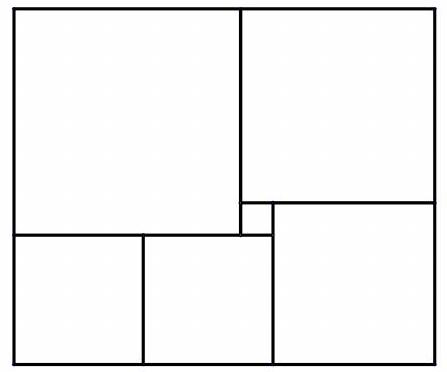
\includegraphics[max width=\textwidth, center]{2024_11_21_a1bccce644610f08c774g-1}


\end{document}